\documentclass[border=4pt]{standalone}
\usepackage{tikz}
\begin{document}

\noindent
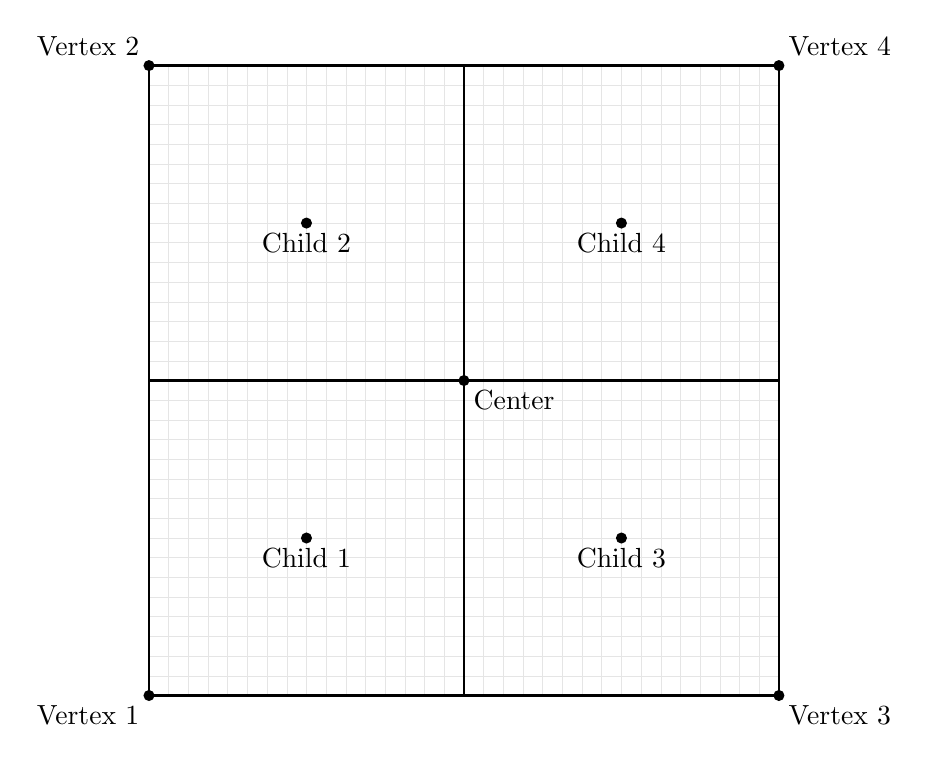
\begin{tikzpicture}[x=0.25cm,y=0.25cm,text centered]
  \draw[step=1,black!10,very thin] (0.0,0.0) grid (32.0,32.0);

  \draw[thick] (0,0) rectangle (32,32);
  \fill (16,16) circle(2pt);
  \node (1616) at (16,16) [below right]  {Center};

  \fill (0,0) circle(2pt);
  \node (0000) at (0,0) [below left]  {Vertex 1};
  \fill (0,32) circle(2pt);
  \node (0032) at (0,32) [above left]  {Vertex 2};
  \fill (32,0) circle(2pt);
  \node (3200) at (32,0) [below right]  {Vertex 3};
  \fill (32,32) circle(2pt);
  \node (3232) at (32,32) [above right]  {Vertex 4};

  \draw[thick] (0,0) rectangle (16,16);
  \fill (8,8) circle(2pt);
  \node (0808) at (8,8) [below]  {Child 1};

  \draw[thick] (0,16) rectangle (16,32); 
  \fill (8,24) circle(2pt);  
  \node (0824) at (8,24) [below]  {Child 2};

  \draw[thick] (16,0) rectangle (32,16);
  \fill (24,8) circle(2pt);  
  \node (2408) at (24,8) [below]  {Child 3};

  \draw[thick] (16,16) rectangle (32,32);
  \fill (24,24) circle(2pt);  
  \node (1616) at (24,24) [below]  {Child 4};

\end{tikzpicture}

\end{document}




